\documentclass[14pt]{extbook}
\usepackage{multicol, enumerate, enumitem, hyperref, color, soul, setspace, parskip, fancyhdr} %General Packages
\usepackage{amssymb, amsthm, amsmath, latexsym, units, mathtools} %Math Packages
\everymath{\displaystyle} %All math in Display Style
% Packages with additional options
\usepackage[headsep=0.5cm,headheight=12pt, left=1 in,right= 1 in,top= 1 in,bottom= 1 in]{geometry}
\usepackage[usenames,dvipsnames]{xcolor}
\usepackage{dashrule}  % Package to use the command below to create lines between items
\newcommand{\litem}[1]{\item#1\hspace*{-1cm}\rule{\textwidth}{0.4pt}}
\pagestyle{fancy}
\lhead{Progress Quiz 7}
\chead{}
\rhead{Version C}
\lfoot{6523-2736}
\cfoot{}
\rfoot{test}
\begin{document}

\begin{enumerate}
\litem{
Solve the quadratic equation below. Then, choose the intervals that the solutions belong to, with $x_1 \leq x_2$ (if they exist).\[ 18x^{2} -11 x -8 = 0 \]\begin{enumerate}[label=\Alph*.]
\item \( x_1 \in [-27.01, -25.6] \text{ and } x_2 \in [25.82, 27.31] \)
\item \( x_1 \in [-0.48, -0.21] \text{ and } x_2 \in [0.98, 1.2] \)
\item \( x_1 \in [-1.14, -0.7] \text{ and } x_2 \in [0.01, 0.62] \)
\item \( x_1 \in [-8.5, -7.69] \text{ and } x_2 \in [17.7, 19.14] \)
\item \( \text{There are no Real solutions.} \)

\end{enumerate} }
\litem{
Solve the quadratic equation below. Then, choose the intervals that the solutions belong to, with $x_1 \leq x_2$ (if they exist).\[ 18x^{2} +12 x -5 = 0 \]\begin{enumerate}[label=\Alph*.]
\item \( x_1 \in [-1.29, -0.77] \text{ and } x_2 \in [-1, 0.8] \)
\item \( x_1 \in [-0.77, -0.07] \text{ and } x_2 \in [0.9, 2.6] \)
\item \( x_1 \in [-17.51, -17.04] \text{ and } x_2 \in [3.9, 5.6] \)
\item \( x_1 \in [-22.98, -22.17] \text{ and } x_2 \in [21, 24.6] \)
\item \( \text{There are no Real solutions.} \)

\end{enumerate} }
\litem{
Solve the quadratic equation below. Then, choose the intervals that the solutions $x_1$ and $x_2$ belong to, with $x_1 \leq x_2$.\[ 25x^{2} +50 x + 24 = 0 \]\begin{enumerate}[label=\Alph*.]
\item \( x_1 \in [-2.55, -2.29] \text{ and } x_2 \in [-0.46, -0.24] \)
\item \( x_1 \in [-2.02, -1.49] \text{ and } x_2 \in [-0.74, -0.46] \)
\item \( x_1 \in [-6.7, -5.06] \text{ and } x_2 \in [-0.39, -0.07] \)
\item \( x_1 \in [-1.3, -0.91] \text{ and } x_2 \in [-0.94, -0.78] \)
\item \( x_1 \in [-30.47, -29.65] \text{ and } x_2 \in [-20.03, -19.8] \)

\end{enumerate} }
\litem{
Graph the equation below.\[ f(x) = (x-4)^2 - 20 \]\begin{enumerate}[label=\Alph*.]
\begin{multicols}{2}\item 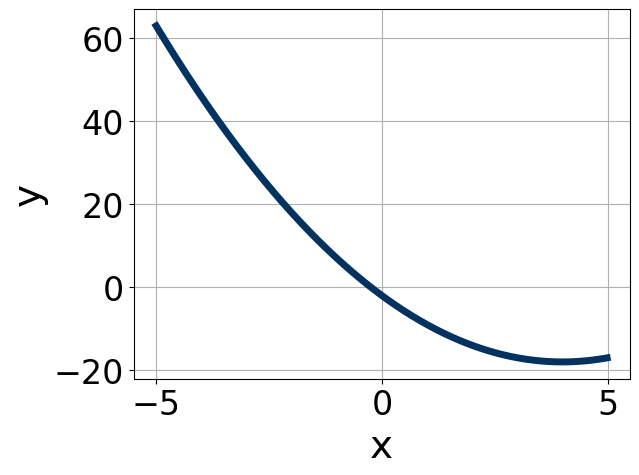
\includegraphics[width = 0.3\textwidth]{../Figures/quadraticEquationToGraphAC.png}\item 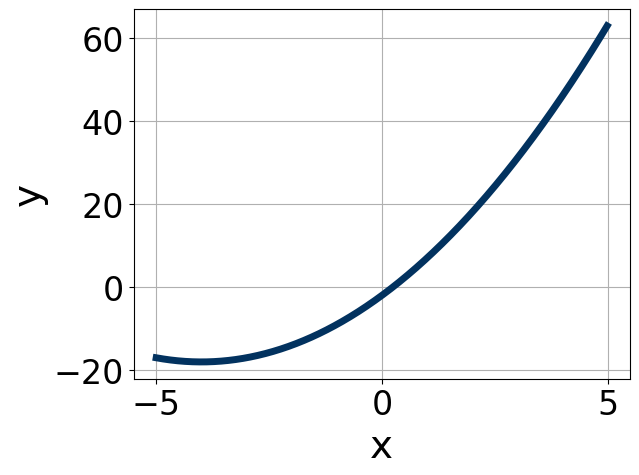
\includegraphics[width = 0.3\textwidth]{../Figures/quadraticEquationToGraphBC.png}\item 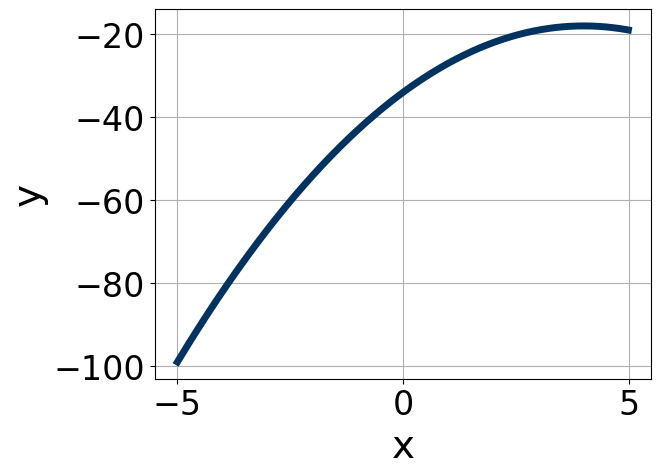
\includegraphics[width = 0.3\textwidth]{../Figures/quadraticEquationToGraphCC.png}\item 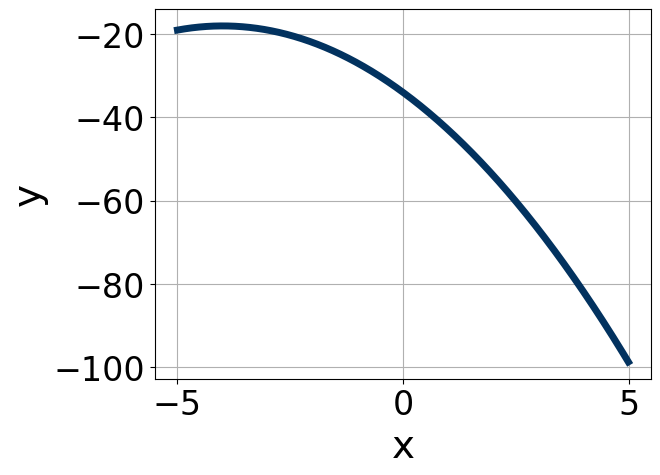
\includegraphics[width = 0.3\textwidth]{../Figures/quadraticEquationToGraphDC.png}\end{multicols}\item None of the above.
\end{enumerate} }
\litem{
Factor the quadratic below. Then, choose the intervals that contain the constants in the form $(ax+b)(cx+d); b \leq d.$\[ 36x^{2} +60 x + 25 \]\begin{enumerate}[label=\Alph*.]
\item \( a \in [0.8, 2.35], \hspace*{5mm} b \in [30, 31], \hspace*{5mm} c \in [-1.2, 2.5], \text{ and } \hspace*{5mm} d \in [28, 32] \)
\item \( a \in [11.56, 12.87], \hspace*{5mm} b \in [-2, 10], \hspace*{5mm} c \in [2.2, 5.1], \text{ and } \hspace*{5mm} d \in [1, 13] \)
\item \( a \in [5.67, 6.37], \hspace*{5mm} b \in [-2, 10], \hspace*{5mm} c \in [4.1, 8.3], \text{ and } \hspace*{5mm} d \in [1, 13] \)
\item \( a \in [2.78, 4.14], \hspace*{5mm} b \in [-2, 10], \hspace*{5mm} c \in [8.6, 14.2], \text{ and } \hspace*{5mm} d \in [1, 13] \)
\item \( \text{None of the above.} \)

\end{enumerate} }
\litem{
Factor the quadratic below. Then, choose the intervals that contain the constants in the form $(ax+b)(cx+d); b \leq d.$\[ 36x^{2} -61 x + 20 \]\begin{enumerate}[label=\Alph*.]
\item \( a \in [1.55, 2.96], \hspace*{5mm} b \in [-6, 2], \hspace*{5mm} c \in [14.5, 18.7], \text{ and } \hspace*{5mm} d \in [-9, -2] \)
\item \( a \in [0.97, 1.75], \hspace*{5mm} b \in [-45, -39], \hspace*{5mm} c \in [-3.7, 1.4], \text{ and } \hspace*{5mm} d \in [-19, -15] \)
\item \( a \in [11.74, 12.53], \hspace*{5mm} b \in [-6, 2], \hspace*{5mm} c \in [2.5, 3.4], \text{ and } \hspace*{5mm} d \in [-9, -2] \)
\item \( a \in [2.5, 5.2], \hspace*{5mm} b \in [-6, 2], \hspace*{5mm} c \in [6.6, 10.1], \text{ and } \hspace*{5mm} d \in [-9, -2] \)
\item \( \text{None of the above.} \)

\end{enumerate} }
\litem{
Graph the equation below.\[ f(x) = -(x-2)^2 + 11 \]\begin{enumerate}[label=\Alph*.]
\begin{multicols}{2}\item 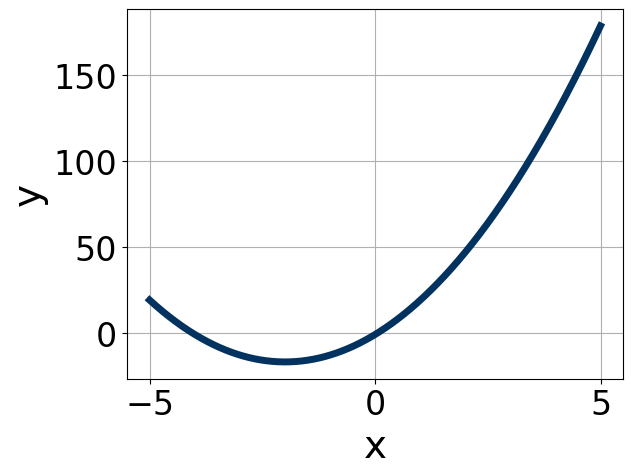
\includegraphics[width = 0.3\textwidth]{../Figures/quadraticEquationToGraphCopyAC.png}\item 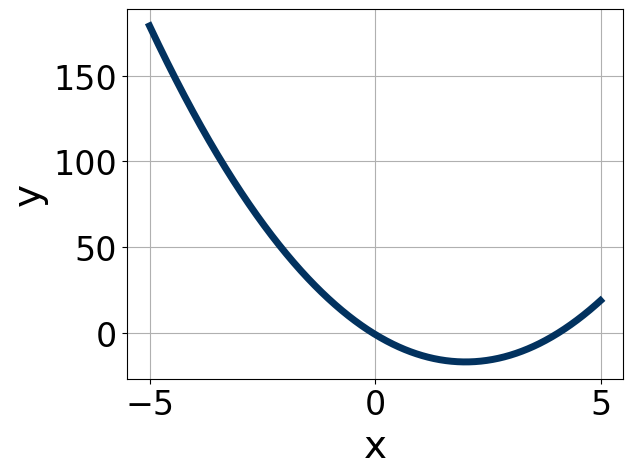
\includegraphics[width = 0.3\textwidth]{../Figures/quadraticEquationToGraphCopyBC.png}\item 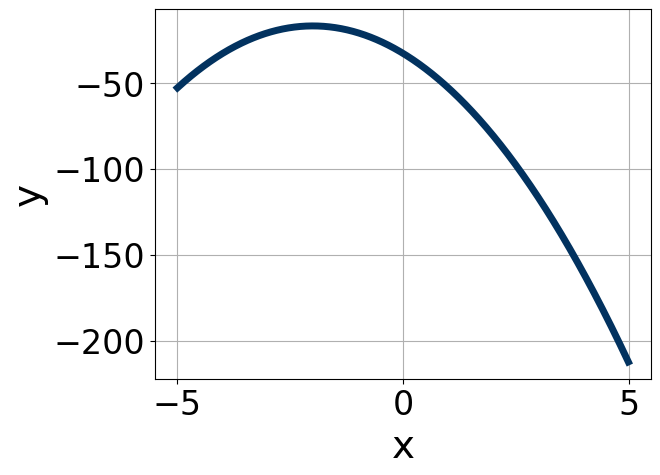
\includegraphics[width = 0.3\textwidth]{../Figures/quadraticEquationToGraphCopyCC.png}\item 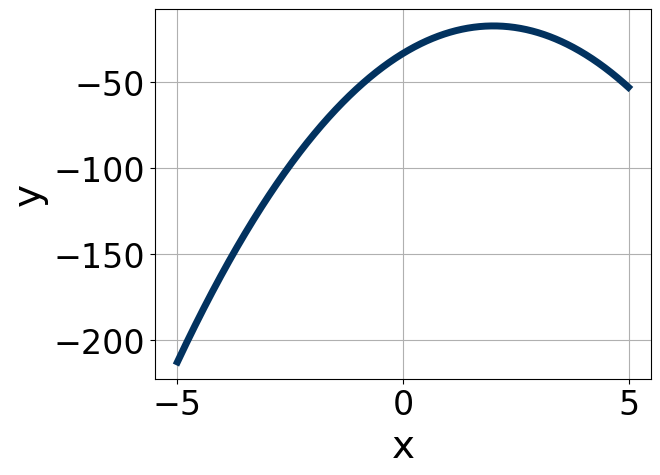
\includegraphics[width = 0.3\textwidth]{../Figures/quadraticEquationToGraphCopyDC.png}\end{multicols}\item None of the above.
\end{enumerate} }
\litem{
Solve the quadratic equation below. Then, choose the intervals that the solutions $x_1$ and $x_2$ belong to, with $x_1 \leq x_2$.\[ 25x^{2} +50 x + 24 = 0 \]\begin{enumerate}[label=\Alph*.]
\item \( x_1 \in [-2.75, -2.08] \text{ and } x_2 \in [-0.47, -0.38] \)
\item \( x_1 \in [-1.24, -0.86] \text{ and } x_2 \in [-1.09, -0.71] \)
\item \( x_1 \in [-30.1, -29.52] \text{ and } x_2 \in [-20.09, -19.88] \)
\item \( x_1 \in [-6.17, -5.8] \text{ and } x_2 \in [-0.29, 0.02] \)
\item \( x_1 \in [-1.77, -1.22] \text{ and } x_2 \in [-0.65, -0.41] \)

\end{enumerate} }
\litem{
Write the equation of the graph presented below in the form $f(x)=ax^2+bx+c$, assuming  $a=1$ or $a=-1$. Then, choose the intervals that $a, b,$ and $c$ belong to.
\begin{center}
    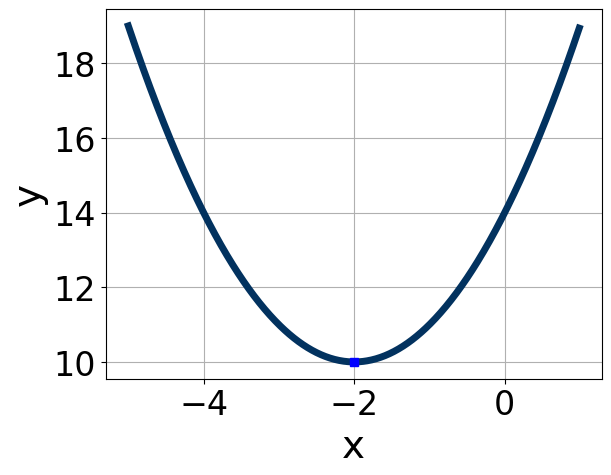
\includegraphics[width=0.5\textwidth]{../Figures/quadraticGraphToEquationCopyC.png}
\end{center}
\begin{enumerate}[label=\Alph*.]
\item \( a \in [0, 4], \hspace*{5mm} b \in [-5, -1], \text{ and } \hspace*{5mm} c \in [6, 8] \)
\item \( a \in [0, 4], \hspace*{5mm} b \in [3, 8], \text{ and } \hspace*{5mm} c \in [2, 3] \)
\item \( a \in [-1, 0], \hspace*{5mm} b \in [3, 8], \text{ and } \hspace*{5mm} c \in [-3, 0] \)
\item \( a \in [0, 4], \hspace*{5mm} b \in [3, 8], \text{ and } \hspace*{5mm} c \in [6, 8] \)
\item \( a \in [-1, 0], \hspace*{5mm} b \in [-5, -1], \text{ and } \hspace*{5mm} c \in [-3, 0] \)

\end{enumerate} }
\litem{
Write the equation of the graph presented below in the form $f(x)=ax^2+bx+c$, assuming  $a=1$ or $a=-1$. Then, choose the intervals that $a, b,$ and $c$ belong to.
\begin{center}
    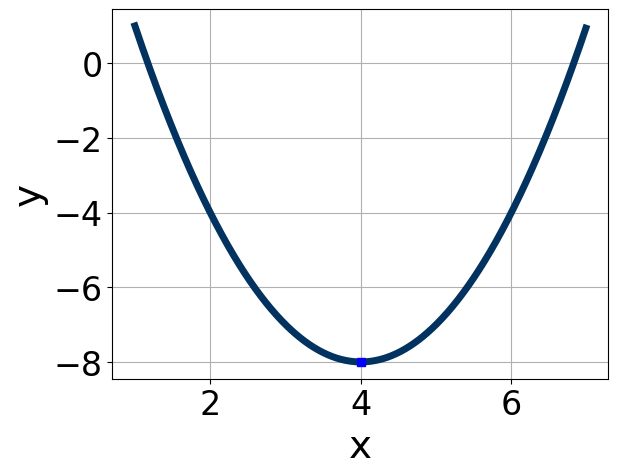
\includegraphics[width=0.5\textwidth]{../Figures/quadraticGraphToEquationC.png}
\end{center}
\begin{enumerate}[label=\Alph*.]
\item \( a \in [-1.4, -0.9], \hspace*{5mm} b \in [6, 11], \text{ and } \hspace*{5mm} c \in [-27, -25] \)
\item \( a \in [0.3, 2.1], \hspace*{5mm} b \in [-12, -6], \text{ and } \hspace*{5mm} c \in [24, 30] \)
\item \( a \in [-1.4, -0.9], \hspace*{5mm} b \in [-12, -6], \text{ and } \hspace*{5mm} c \in [-27, -25] \)
\item \( a \in [0.3, 2.1], \hspace*{5mm} b \in [6, 11], \text{ and } \hspace*{5mm} c \in [4, 9] \)
\item \( a \in [0.3, 2.1], \hspace*{5mm} b \in [-12, -6], \text{ and } \hspace*{5mm} c \in [4, 9] \)

\end{enumerate} }
\end{enumerate}

\end{document}